\section{Preprocesamiento de datos en dos etapas}\label{sec:segunda}

En este artículo se utiliza un enfoque novedoso de preprocesamiento de datos en dos etapas que incorpora tanto la selección de características como la reducción de instancias propuesto en \cite{liu_empirical_2015}. Específicamente, en la etapa de selección de características, primero realizamos un análisis de relevancia y luego proponemos un método de agrupamiento basado en umbrales, llamado algoritmo de agrupamiento basado en umbrales, para realizar el control de redundancia. En la etapa de reducción de instancias, aplicamos submuestreo aleatorio para mantener el equilibrio entre las instancias defectuosas y no defectuosas.

\subsection{Etapa de selección de características}

El primer paso es realizar un análisis de relevancia para eliminar las características irrelevantes y el segundo paso es realizar un control de redundancia para eliminar las características redundantes. 

\begin{figure}[h!]
    \centering
    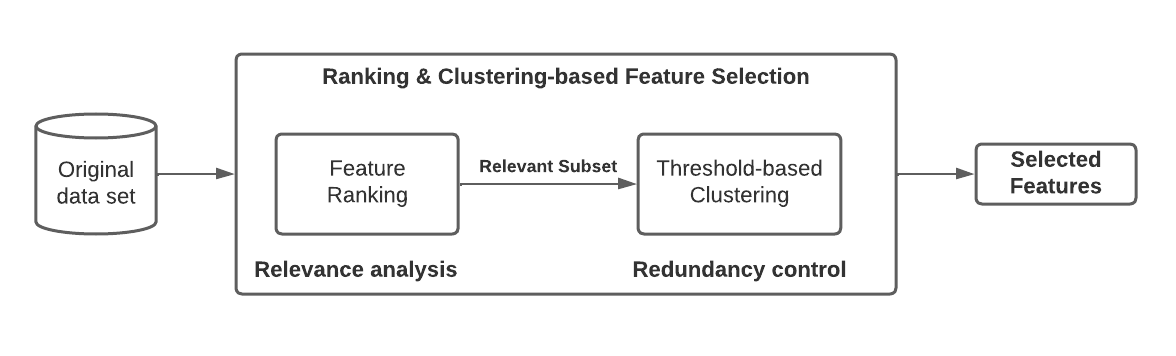
\includegraphics[width=\textwidth]{figs/etapas/Imagen1.png}
    \setstretch{1} %Interlineado 1
	\captionsetup{labelsep=period, labelfont=bf}
    \caption{Detalle de los pasos del modelo de selección}
    \label{fig:logos}
\end{figure}

\subsubsection{Análisis de relevancia}

En el proceso de clasificación, la relevancia de las características individuales se evalúa en el primer paso. Este análisis implica clasificar las características según su importancia o pesos, que son cruciales para diferenciar instancias entre diversas clases (por ejemplo, Bug o NoBug). Para este propósito, se adopta una representación específica de cada grupo, como se describe en \cite{chen_empirical_2013}.



\begin{itemize}
\item Ganancia de información (IG): La idea detrás de este algoritmo es que las características que proporcionan la mayor ganancia de información son las más útiles para la tarea de clasificación o predicción que estamos realizando.

La fórmula matemática para calcular la ganancia de información es la siguiente:

Ganancia de información = Entropía inicial - Entropía final

Donde la entropía inicial es la entropía del conjunto de datos antes de utilizar la característica para dividir el conjunto en subconjuntos más pequeños, y la entropía final es la suma de las entropías de cada subconjunto después de dividir el conjunto de datos utilizando la característica.

La entropía se calcula utilizando la siguiente fórmula:
\begin{equation}
\text{Entropía} = - \sum_{x} p(x) \log_{2}\left(p(x)\right)
	\label{eq:entropia}
\end{equation}

Donde p(x) es la probabilidad de que una observación pertenezca a la clase x.

\item Chi-Cuadrado (CS): El algoritmo Chi-Cuadrado es una técnica estadística utilizada para evaluar si existe una relación entre dos variables categóricas.

 Para calcular el valor Chi-Cuadrado, comparamos la distribución esperada con la distribución observada, es decir, con los valores reales de cada combinación de valores de A y B en nuestro conjunto de datos. Si la diferencia entre la distribución esperada y la observada es significativamente grande, podemos concluir que existe una relación entre las dos variables.

La fórmula para calcular el valor Chi-Cuadrado es la siguiente:
\begin{equation}
\text{Chi-Cuadrado} = \sum \frac{(O - E)^{2}}{E}
	\label{eq:chisqr}
\end{equation}

\item ReliefF (RF): A diferencia de otros algoritmos de selección de características, como la ganancia de información o el algoritmo Chi-Cuadrado, ReliefF tiene en cuenta la relación entre las características y las etiquetas o clases en el conjunto de datos.

El algoritmo ReliefF utiliza la distancia para evaluar cuánto aporta cada característica a la tarea de clasificación o predicción. Para ello, selecciona una observación aleatoriamente y luego busca las observaciones más cercanas y más lejanas en el espacio de características. Luego, calcula la diferencia entre la distancia a la observación más cercana y la distancia a la observación más lejana para cada característica y utiliza esta información para asignar un peso a cada característica. Las características con pesos más altos son las más importantes para la tarea de clasificación o predicción.

La fórmula matemática utilizada en el algoritmo ReliefF para asignar pesos a las características es la siguiente:

Peso de la característica i = (distancia a la observación más cercana de la misma clase - distancia a la observación más cercana de otra clase) / número de observaciones seleccionadas aleatoriamente.
\end{itemize}

\subsection{Control de redundancia}
El algoritmo de agrupamiento basado en umbrales (NTC) se utiliza para el segundo paso. En \cite{liu_empirical_2015} se encuentra un seudocódigo del algoritmo NTC.  Al principio, las funciones se agrupan en clústeres utilizando un umbral preespecificado. Para agrupar estas características, el algoritmo comienza calculando la similitud entre cada par de características y construye un gráfico de vecino más cercano sobre las características. Este proceso se repite y se van eliminando o seleccionando las características que cumplan con el umbral definido para la ejecución. Los métodos para calcular la similitud entre cualquier par de características se describirán a continuación \cite{liu_empirical_2015,chen_empirical_2013}.

\begin{itemize}
\item Incertidumbre simétrica (SU): La incertidumbre simétrica mide el coeficiente de entropía entre dos variables aleatorias y muchos investigadores la han utilizado para evaluar la similitud entre características \cite{yu2003feature,liu_empirical_2015}.
\item Semejanza de coseno (COS): La similitud de coseno mide el coseno del ángulo entre dos vectores euclidianos, construido por los valores de las dos características según el orden de instancia \cite{liu_empirical_2015}.
\end{itemize}

\subsection{Métodos de balanceo de número instancias}

\textbf{Random Under Sampling (RUS)} es una técnica de remuestreo utilizada en el aprendizaje automático para tratar el problema de desequilibrio de clases. El objetivo de RUS es reducir la cantidad de muestras de las clases sobre-representadas (o mayoritarias) de tal manera que se iguale la cantidad de muestras de las clases sub-representadas (o minoritarias) \cite{junsomboon_combining_2017,hossen_hybrid_2020}.

La manera en que se lleva a cabo el RUS es mediante la eliminación aleatoria de muestras de las clases mayoritarias. Esto se hace de forma que la proporción de muestras de las clases mayoritarias y minoritarias se acerque a una proporción deseada. Por ejemplo, si se quiere que la proporción de muestras de las clases mayoritarias y minoritarias sea 1:1, entonces se eliminarán aleatoriamente la mitad de las muestras de la clase mayoritaria.

Estas técnicas se utilizan a menudo cuando hay una desproporción significativa entre las diferentes clases en un conjunto de datos, lo que puede afectar negativamente a la precisión de los modelos de aprendizaje automático entrenados con este conjunto de datos.

En resumen, la técnica de Random Under Sampling busca balancear la proporción de muestras entre las diferentes clases reduciendo el tamaño de las clases mayoritarias.


\textbf{Random Over Sampling (ROS)} es una técnica de remuestreo utilizada en el aprendizaje automático para tratar el problema de desequilibrio de clases. El objetivo de ROS es aumentar la cantidad de muestras de las clases sub-representadas (o minoritarias) de tal manera que se iguale la cantidad de muestras de las clases sobre-representadas (o mayoritarias)  \cite{junsomboon_combining_2017,hossen_hybrid_2020}.

La manera en que se lleva a cabo el ROS es mediante la duplicación aleatoria, con reemplazo, de instancias existentes de las clases minoritarias; a diferencia de SMOTE, no crea instancias nuevas. Esto se hace de forma que la proporción de muestras de las clases mayoritarias y minoritarias se acerque a una proporción deseada. Por ejemplo, si se quiere una proporción 1:1, se duplican instancias de la clase minoritaria hasta igualar el número de instancias de la clase mayoritaria.

En resumen, la técnica de Random Over Sampling busca balancear la proporción de muestras entre las diferentes clases aumentando el tamaño de las clases minoritarias mediante la duplicación de instancias existentes.


\textbf{SMOTE (Synthetic Minority Over-sampling Technique)} es una técnica utilizada en Machine Learning para abordar el problema del desequilibrio de clases. Su objetivo es equilibrar la distribución de clases creando muestras sintéticas de la clase minoritaria. A continuación, se separa la explicación en la parte lógica matemática y el detalle del funcionamiento de SMOTE:



\textbf{Parte Lógica Matemática:}
\begin{enumerate}
\item \textbf{Detección de la Clase Minoritaria:} El primer paso es identificar la clase minoritaria en el conjunto de datos de clasificación, es decir, la clase que tiene menos ejemplos.
\item \textbf{Selección de Vecinos:} Para cada instancia de la clase minoritaria, SMOTE selecciona k vecinos cercanos. El valor de k se establece previamente.
\item \textbf{Generación de Muestras Sintéticas:} Para cada instancia de la clase minoritaria, SMOTE crea nuevas muestras sintéticas interpolando características entre la instancia original y sus vecinos seleccionados. La fórmula general es:


\begin{equation}
\fontsize{12}{9}\selectfont
\text{Nueva Muestra} = \text{Instancia Original} + (\text{Vecino} - \text{Instancia Original}) \times \text{ratio}
	\label{eq:smote}
\end{equation}

   Donde \textbf{ratio} es un valor entre 0 y 1 que determina cuánto se debe mover hacia el vecino para crear la nueva muestra.
\end{enumerate}

\textbf{Detalle del Funcionamiento:}
\begin{enumerate}
\item \textbf{Detección de la Clase Minoritaria:} SMOTE comienza identificando cuál es la clase minoritaria en el conjunto de datos. Esto se hace para asegurarse de que las nuevas muestras sintéticas se generen solo para esta clase.
\item \textbf{Selección de Vecinos:} Para cada instancia de la clase minoritaria, SMOTE elige al azar k vecinos cercanos. El valor de k se elige previamente por el usuario.
\item \textbf{Generación de Muestras Sintéticas:} Para cada instancia de la clase minoritaria, se sigue el proceso de generación de muestras sintéticas:
    \begin{enumerate}
        \item Se selecciona una instancia de la clase minoritaria.
        \item Se elige uno de sus k vecinos cercanos al azar.
        \item Se calcula un valor de 'ratio' entre 0 y 1, que determina cuánto se moverá desde la instancia original hacia el vecino. El valor de 'ratio' se elige al azar.
        \item Se utiliza la fórmula mencionada anteriormente para generar una nueva muestra sintética, que se suma a la clase minoritaria.
    \end{enumerate}
\item \textbf{Repetición:} Este proceso se repite hasta que se alcance un equilibrio deseado entre las clases o hasta que se alcance un número específico de muestras sintéticas generadas.
\end{enumerate}

SMOTE es una técnica efectiva para abordar el desequilibrio de clases, ya que aumenta el tamaño de la clase minoritaria de manera artificial, lo que puede ayudar a que los modelos de Machine Learning tengan un mejor rendimiento al tratar con datos balanceados. Sin embargo, también es importante tener en cuenta que SMOTE puede introducir ruido en los datos, ya que las muestras sintéticas se generan mediante interpolación y no representan datos reales observados. Por lo tanto, es importante evaluar el impacto de SMOTE en el rendimiento del modelo y considerar otras estrategias de manejo de datos desequilibrados según sea necesario.



\subsection{Modelos de clasificación} \label{sub:modelos}

En el estudio principal se utiliza el modelo de clasificación Random Forest (RF) en la herramienta Weka para realizar los experimentos con los diferentes conjuntos de datos. En el análisis de sensibilidad (Sección \ref{sec:sensibilidad}) se utilizan, además, XGBoost y una SVM lineal, junto con Random Forest, implementados en \textit{scikit-learn}; estos algoritmos se describen en la Sección \ref{sec:clasificadores_mt}.

RF: basado en un conjunto de árboles de decisiones. En su funcionamiento se utilizan algunas ecuaciones matemáticas, como las utilizadas en la construcción de un árbol de decisiones individual, como Gini impurity, Information Gain o Reduction in Variance \cite{shah_comparative_2020}.

La idea principal de RF es la creación de un gran número de árboles de decisiones, cada uno de ellos construido con un subconjunto de datos de entrenamiento y un subconjunto de características, y luego se combina los resultados de todos los árboles para tomar una decisión final.

El proceso de selección de características para cada árbol se realiza mediante un procedimiento conocido como "bagging" (Bootstrap Aggregating) y selección aleatoria de características, esto permite reducir la varianza y mejorar la precisión del modelo.

En resumen, el algoritmo RF se basa en la combinación de un gran número de árboles de decisiones construidos de manera aleatoria, utilizando las ecuaciones matemáticas ya mencionadas para medir la impureza o la reducción de incertidumbre en cada rama del árbol.


